\documentclass{beamer}
\setbeamertemplate{navigation symbols}{}
\setbeamertemplate{caption}{\insertcaption}

\usetheme{Dresden}
%\usecolortheme{albatross}
%\usecolortheme{beaver}
%\usecolortheme{beetle}
%\usecolortheme{crane}
%\usecolortheme{dolphin}
%\usecolortheme{dove}
%\usecolortheme{fly}
%\usecolortheme{lily}
\usecolortheme{orchid}
%\usecolortheme{rose}
%\usecolortheme{seagull}
%\usecolortheme{seahorse}
%\usecolortheme{whale}
%\usecolortheme{wolverine}

\usepackage{amsmath}
\graphicspath{{figs/}}
\usepackage{multirow}

\usepackage{tikz}

\let\Tiny\tiny
\usepackage{graphicx}
\usepackage{xmpmulti}
\usepackage{multimedia}
%\usepackage{media9}


\beamersetuncovermixins{\opaqueness<1>{25}}{\opaqueness<2->{15}}

\begin{document}
	\title{Machine Learning}  
	\author{Saumya Bhatnagar}
	\date{\today} 
	
	
\begin{frame}
\titlepage
\end{frame}

\begin{frame}[allowframebreaks]\frametitle{Table of contents}\tableofcontents
\end{frame} 




\section{EDA}

\subsection{General}
\begin{frame}\frametitle{Box cox transformation}
	convert data to a normal distribution
\end{frame}

\begin{frame}\frametitle{CRISP-DM}
Cross-industry standard process for data mining
\end{frame}

\begin{frame}\frametitle{Dimensionality Reduction}
\begin{itemize}
	\item PCA: is a linear method
	\item \hyperlink{rf}{Random Forest}
\end{itemize}
\end{frame}

\begin{frame}\frametitle{Cross-Validation Techniques}
	\textbf{why cross-validation?}\\
	\begin{enumerate}
		\item LOOCV (leave one out cv): $\downarrow$ bias, $\uparrow$variability\\n MSEs
		\item k-fold: $\uparrow$k =$\Rightarrow$ $\downarrow$Variance; $\downarrow$bias; (generally k=10 with 10 MSEs)
		\item stratified CV: $\downarrow$Variance \& $\downarrow$bias\\
		uses stratified sampling for each fold
		\item forward chaining or rolling origin
	\end{enumerate}
\end{frame}



\subsection{General2}

\begin{frame}\frametitle{Under and Over Sampling}
\end{frame}

\begin{frame}\frametitle{Univariate and Multivariate Analysis}
\end{frame}


\begin{frame}\frametitle{Class Imbalance}
\end{frame}

\section{Regression}


\subsection{Types}

\begin{frame}\frametitle{what is regression?}
	Regression analysis is a statistical technique to assess the relationship between an predictor variable and one or more response factors.\\
	http://www.statisticshowto.com/probability-and-statistics/regression-analysis/
	(go to definitions)
\end{frame}


\begin{frame}\frametitle{Linear vs Logistic}
	\begin{columns}
		\begin{column}{0.6\textwidth}
			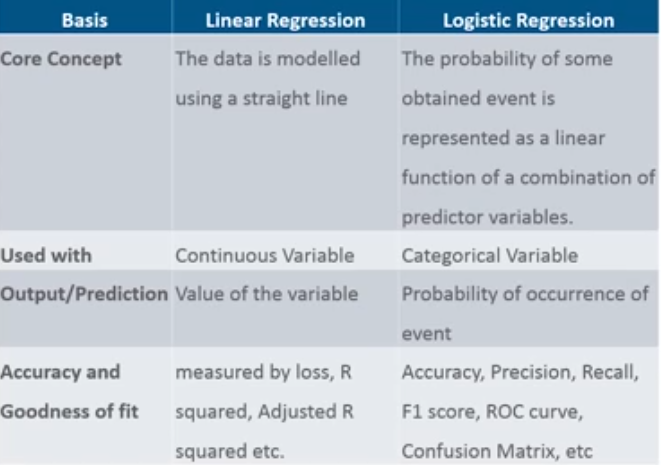
\includegraphics[scale=0.45]{regression/linearlogistic}
		\end{column}
		\begin{column}{0.2\textwidth}
			Data is modelled using a straight line vs using a sigmoid function\\
			maps continuous x to cont y, vs maps cont x to binary y 
		\end{column}
	\end{columns}

\end{frame}

\begin{frame}[plain]%\frametitle{}
\begin{table}[h]
	\centering
	\begin{tabular}{cccc}
		\textbf{Outcome} & \textbf{GLM Family} & \textbf{Link} & \textbf{Mean to} \\
		\textbf{Variable} & & & \textbf{Variance} \\ 
		\hline %\pause 
		Continuous, & Normal or & \\ unbounded & Standard Gaussian & Identity &  \\  
		\hline
		Continuous, & Gamma or & \\ non-negative & inverse Gamma &  &  \\ \hline
		
		
		Discrete/ & Poisson & Log & Identity \\
		counts/ & Quassi-poisson or &  & If not \\
		rate & negative binomial & & Identity \\
		
		
		\hline
		
		Count & Gamma &  & Over dispersion \\ \hline
		Counts with & Zero inflated poisson & \\ multiple zero & may be checked 
		for fitting & & \\ \hline
		Binary & Binomial or & \\  & Logistic regression & & \\ \hline
		Nominal  & Multinomial regression & \\
		\hline
	\end{tabular} 
	\caption{Regression Model Selection Criteria}
\end{table}
\end{frame}

\begin{frame}\frametitle{bias vs variance}
	Linear model: $\theta_0 + x \theta_1 \rightarrow$ increased bias, underfit\\
	Polynomial model: $\theta_0 + \sum {x \theta_n} \rightarrow$ increased variance, overfit\\

	So, \textbf{optimization on training data}, using\\
	\begin{enumerate}
		\item OLS
		\item gradient descent, 
		\item max likelihood estimation (mle)
	\end{enumerate}
	
	Types of Bias:
	\begin{enumerate}
		\item selection bias
		\item survivorship bias (air plane)
		\item under coverage bias
	\end{enumerate}

\end{frame}


\begin{frame}\frametitle{When overfit use Regularization Techniques}
	restrict freedom $\Rightarrow$ regularization\\
	model selection algo\\
	overfit $\Rightarrow$ fail to generalize to new examples\\
	num datapoints > num features or num parameters\\
	reduce magnitude of features by penalization\\
	\begin{tabular}{c|c}
			\textbf{L1 Regularization} & \textbf{L2 Regularization}\\ 
			lasso regression & Ridge regression\\ \hline
				
			Sum of sq residual + $\lambda$ $|$slope$|$
			& Sum of likelihoods + $\lambda$ slope$^2$
			\\ \hline
			can shrink slope to exact 0
			& asymptotically 0
			\\ \hline
			LAR = Least absolute regression 
			& \\
			multiple solution
			& \\ \hline
	\end{tabular}

\end{frame}



\subsection{Linear regression}
\begin{frame}\frametitle{Linear Regression using Least Squares}
	\begin{enumerate}
		\item \textbf{fitting a line to the data}: as shown below\\
		\item Find best fit using \textbf{Least Squares}\\
		sum of squared residuals = $\sum (y-\hat{y})^2$
		\item Find goodness of fit using \textbf{R squared} method\\
		R squared (aka coefficient of determination) is a statistical measure of how well the data fits line\\
		low R squared doesn't always mean bad 
	\end{enumerate}
	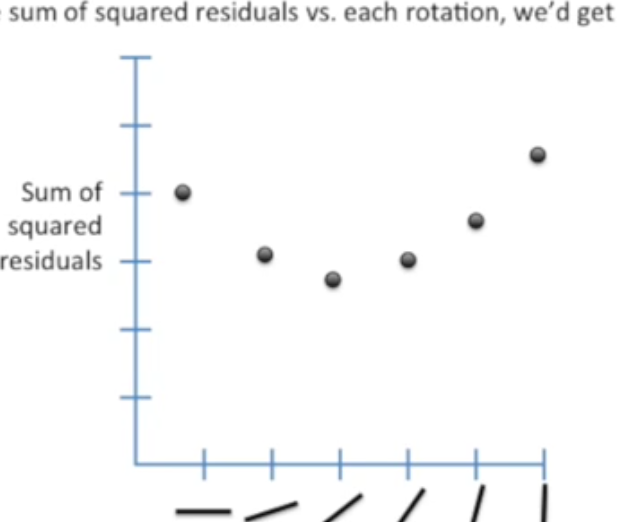
\includegraphics[scale=0.15]{regression/linear}
	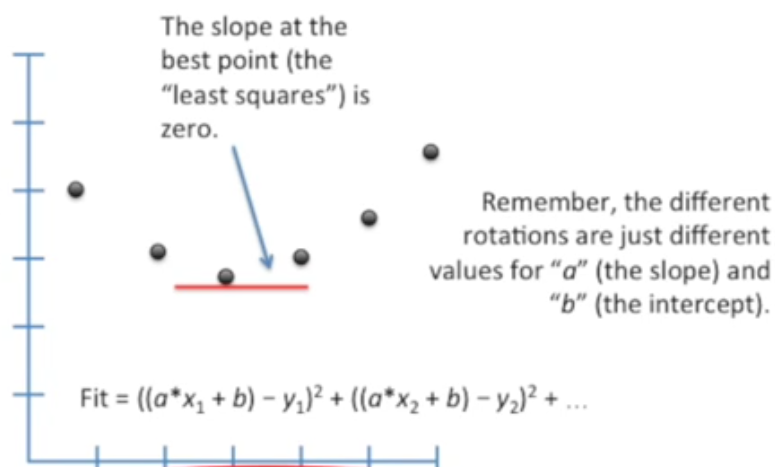
\includegraphics[scale=0.15]{regression/linear2}
	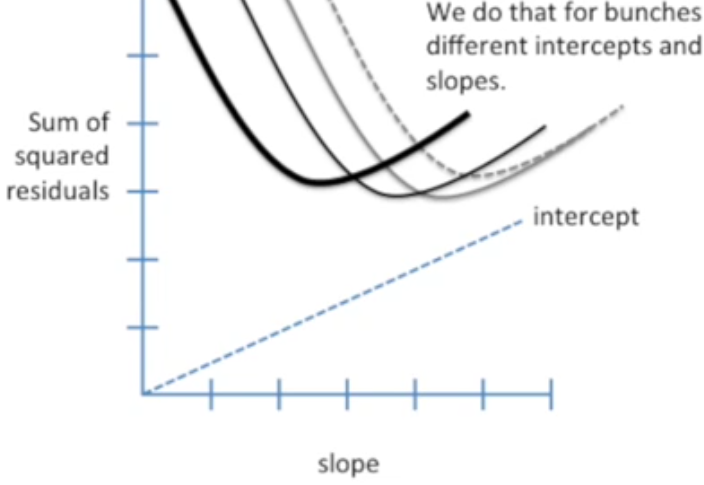
\includegraphics[scale=0.15]{regression/linear3}\\	
\end{frame}


\begin{frame}%\frametitle{manual calculation}
	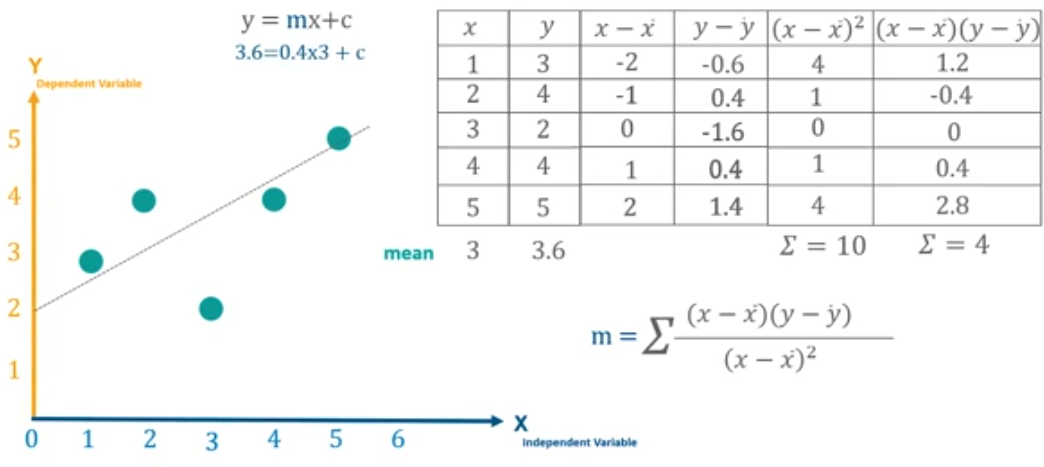
\includegraphics[scale=0.27]{regression/linearmanual}
	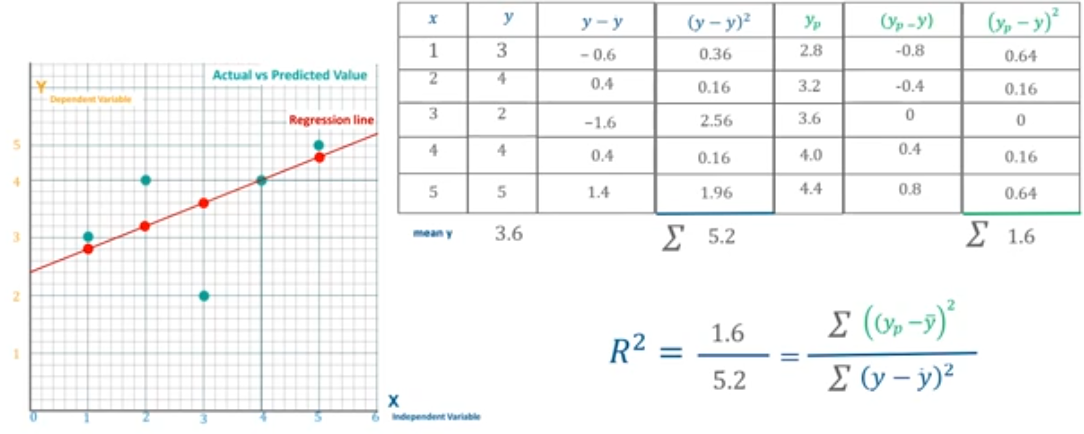
\includegraphics[scale=0.27]{regression/linearmanualrsq}
\end{frame}

\begin{frame}\frametitle{characteristics of Linear Regression}
	outliers have big bad impact\\
	Computational complexity O(n)\\
	comprehensible and transparent
\end{frame}

\begin{frame}\frametitle{Linear vs Multiple Regression}
	\begin{columns}
		\begin{column}{0.5\textwidth}
			\textbf{Linear}\\
			fit line\\
			Calculate R$^2$\\
			$R^2 = \frac{SS(mean_y)-SS(fit)}{SS(mean_y)}$\\
			cal F-score and p-val\\
			$F = \frac{\frac{SS(mean)-SS(fit)}{p_{fit}-p_{mean}}}{\frac{SS(fit)}{n-p_{fit}}}$
		\end{column}
		\begin{column}{0.5\textwidth}
			\textbf{Multiple}\\
			fit plane or higher dimensional\\
			Cal R$^2$\\
			Adjust R$^2$ to compensate for additional parameters\\
		\end{column}
	\end{columns}
\end{frame}

\begin{frame}\frametitle{Multiple Regression}
	\textbf{Fit plane of higher dimensional obj to the data}\\
	
\end{frame}

\subsection{Logistic}
\begin{frame}\frametitle{Logistic Regression}
content...
\end{frame}



%%%%%%%%%%%%%%%%%%%%%%%%%%%%%%%%%%%%%%%%%%%%%%%%%%%%%%%%%%%%%%%%%%%%%%%%%%%%%%%%%%%%%%%%%%%%%%%%%%%%%%%%%%5







\section{Classification}
\begin{frame}
	Three methods to classifier
	\begin{enumerate}
		\item model a classification rule - knn, decision tree, perceptron, svm
		\item model the probability of class membership given input data - perceptron with cross-entropy cost
		\item make a probabilistic model of data within each class - naive bayes
		1 \& 2 are discriminative classifications
		3 is generative classification
		2 \& 3 probabilistic classification
	\end{enumerate}
\end{frame}

\subsection{Decision Tree and Random Forest}
\begin{frame}\frametitle{Decision Tree}
	content...
\end{frame}

\begin{frame}\frametitle{Random Forest}
content...
\end{frame}



\section{Clustering}
\subsection{Clustering Types}
\begin{frame}
	“Help me understand our customers better so that we can market our products to them in a better manner!\\
	\textbf{Monothetic}: Cluster members have some common property\\
	Expectation–Maximization (EM) Clustering using Gaussian Mixture Models (GMM)\\
	\textbf{Polythetic}: Cluster members are similar to each other. Distance between elements define relationship\\
	\textbf{Hard Clustering}: each data point either belongs to a cluster completely or not\\
	\textbf{Soft Clustering}: a probability or likelihood of that data point to be in those clusters is assigned.
\end{frame}

\begingroup
\tiny


\begin{frame}\frametitle{Clustering Models}
\hspace*{-3pt}\makebox[\linewidth][c]{

\begin{tabular}[t]{ p{2.6cm}|p{2.7cm}|p{3.3cm}|p{2.6cm}  }
	\hline
	%\multicolumn{4}{|c|}{Country List} \\
	%\hline
	%\vspace{0pt}
	\textbf{Connectivity models}
	& \textbf{Distribution models}
	&\textbf{Centroid models}
	&\textbf{Density models}\\
	\hline
	data points closer in data space exhibit more similarity to each other than the data points lying farther away & 
	how probable is it that all data points in the cluster belong to the same distribution (e.g: Normal, Gaussian) &
	iterative clustering algorithms in which the notion of similarity is derived by the closeness of a data point to the centroid of the clusters& 
	isolates various different density regions and assign the data points within these regions in the same cluster
	\\ \hline
	hierarchical clustering 
	&Expectation-maximization 
	& K-Means, k-median
	& mean-shift, DBSCAN and OPTICS
	\\ \hline
	Approaches: 1) Top-bottom, 2) bottom-up
	& EM uses multivariate normal distributions 
	& DZA
	& DBSCAN uses radius $\epsilon$ and Center c
	\\ \hline
	lacks scalability for handling big datasets, Time complexity: O(n$^2$)
	& These models often suffer from over-fitting. Prior knowledge to define num clusters
	& important to have prior knowledge of the dataset. results change in every trial 
	& DBSCAN doesn’t perform as well when the clusters are of varying density
	\\ \hline
	Results are reproducible 
	& more flexibility in terms of cluster covariance due to $\mu and \sigma$ (additional \textbf{$\sigma$})
	& can handle big data , Time complexity: O(n)
	& DBSCAN identifies outliers as noises
	\\ \hline 
	chk1 & elliptical shape (since we have a standard deviation in both the x and y directions
	& work well when the shape of the clusters is hyper spherical (like circle in 2D, sphere in 3D)   & DBSCAN: can find arbitrarily sized and arbitrarily shaped clusters
	\\ \hline
	Angola& GMMs support mixed membership since is probability based & AGO&DBSCAN: drawback in high-dimensional data since the distance threshold $\epsilon$ becomes challenging to estimate\\
	\hline
\end{tabular}

}
\end{frame}
\endgroup


\begin{frame}%\frametitle{comparisons}
	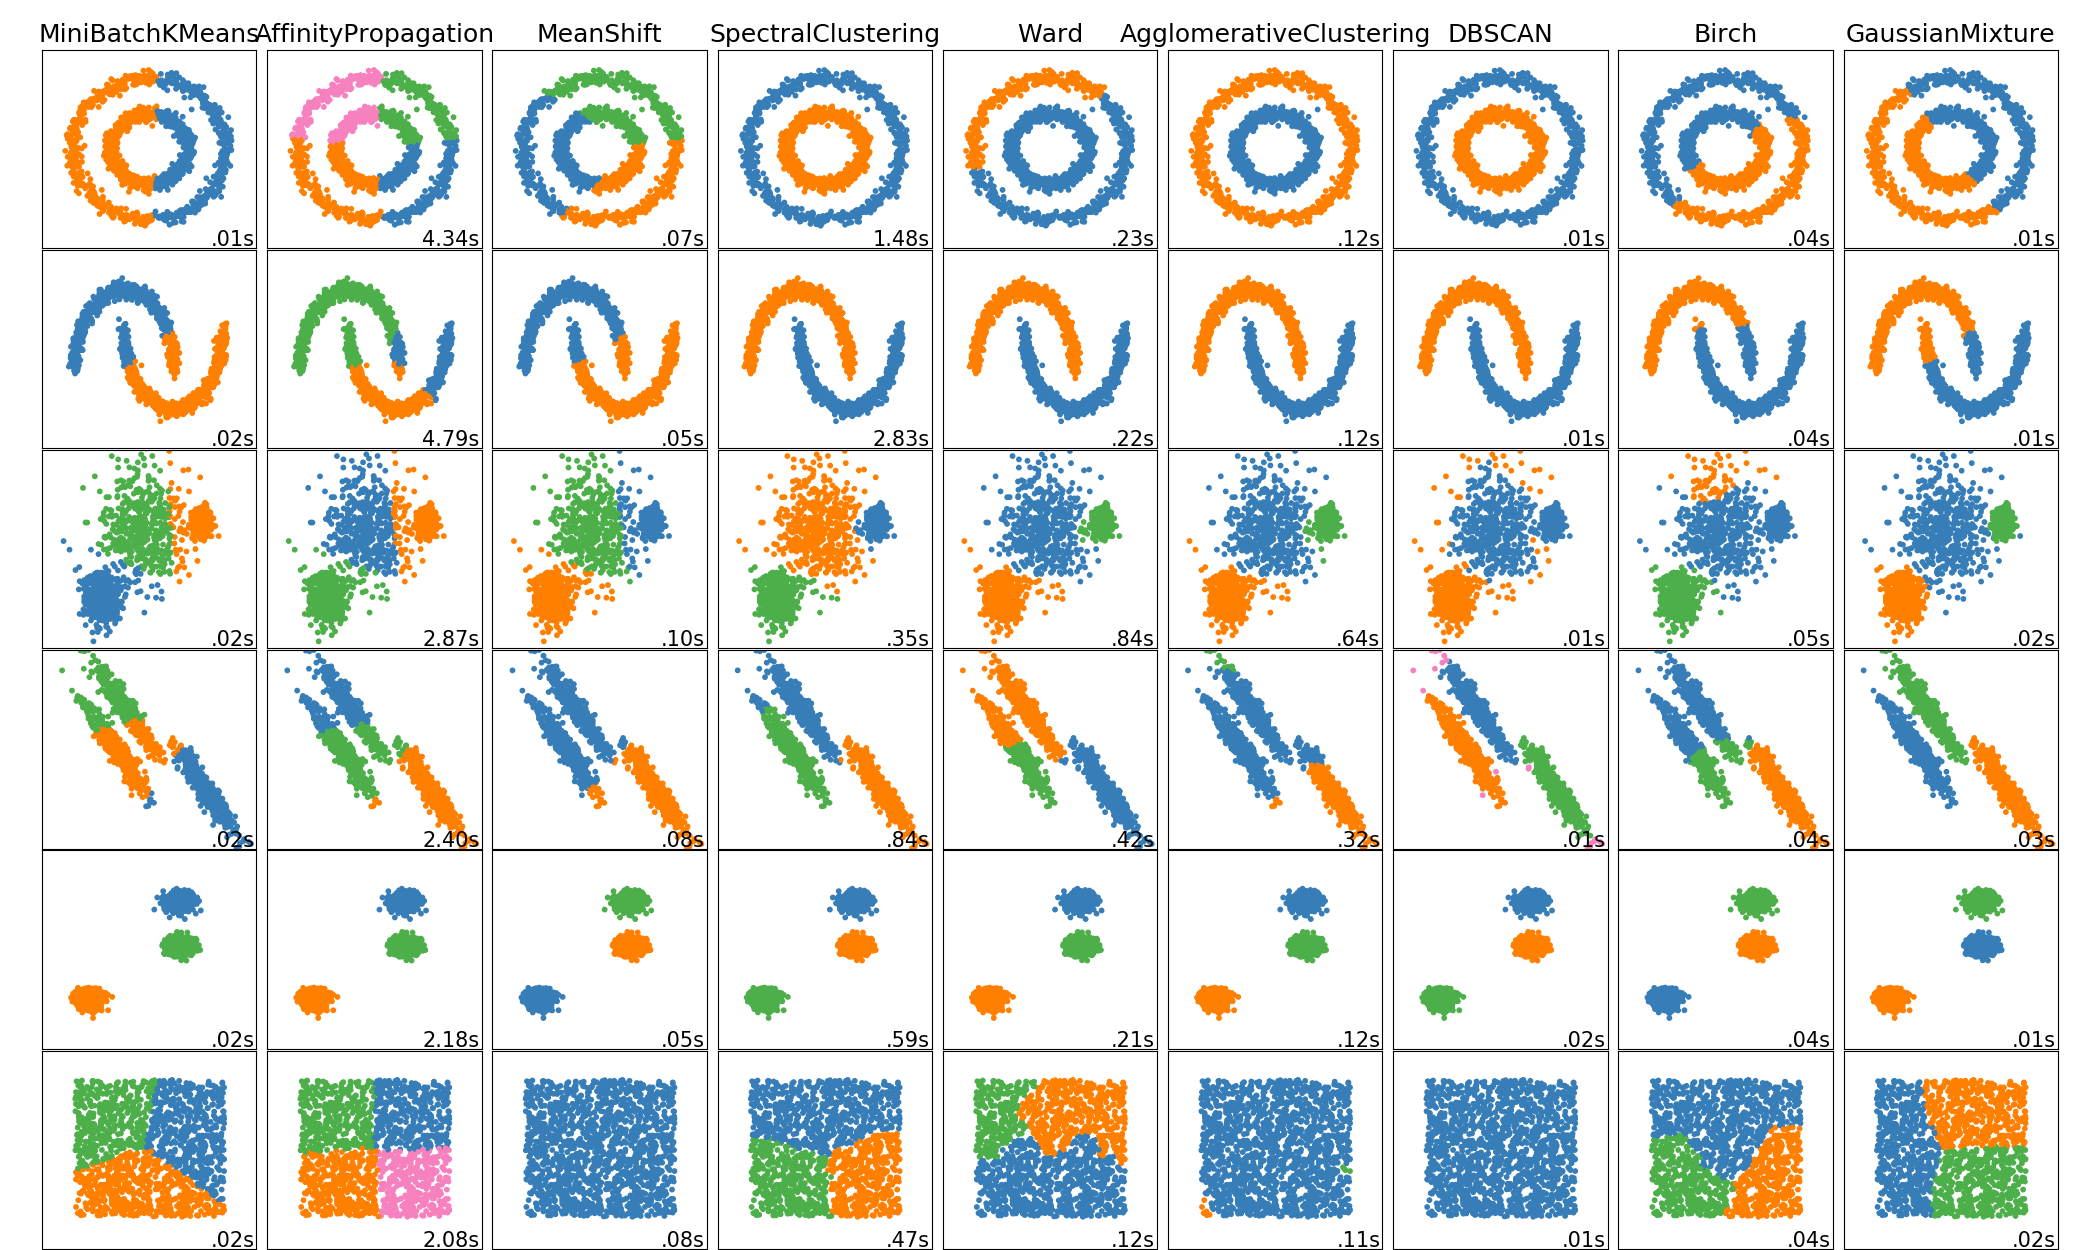
\includegraphics[scale=0.15]{clustering}

\end{frame}




\subsection{Density Models}
\begin{frame}\frametitle{mean-shift clustering}

consider a set of points in two-dimensional space\\
a circular sliding window C centered and radius r as the kernel\\
hill-climbing algorithm that involves shifting this kernel iteratively to a higher density ($\propto$ number of points)  region until convergence\\
At every iteration,\\
- shift the center point to the mean of the points within the window (hence the name)\\
-gradually move towards areas of higher point density\\
- until no longer increase in the density\\
- When multiple sliding windows overlap the window containing the most points is preserved. The data points are then clustered according to the sliding window in which they reside.


\end{frame}


\begin{frame}%\frametitle{meanshift}
\hspace*{-4pt}\makebox[\linewidth][c]{
\begin{tabular}{ccccc}
	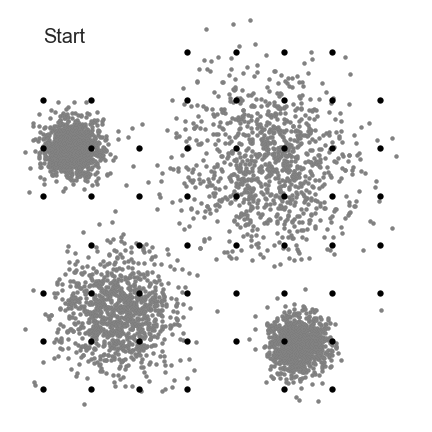
\includegraphics[scale=0.15]{meanshift/meanshift-3}&
	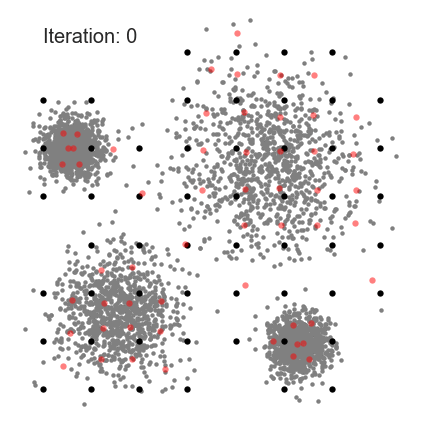
\includegraphics[scale=0.15]{meanshift/meanshift-4}&
	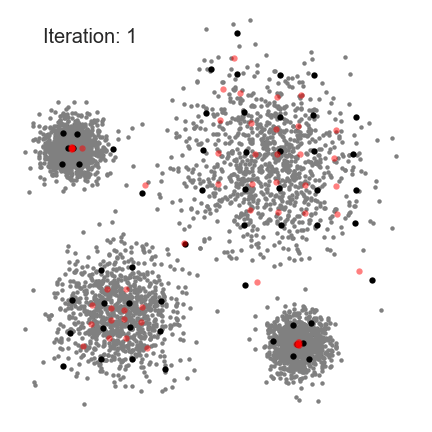
\includegraphics[scale=0.15]{meanshift/meanshift-6}&
	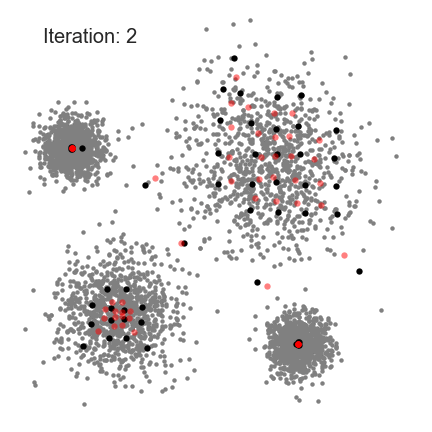
\includegraphics[scale=0.15]{meanshift/meanshift-8}&
	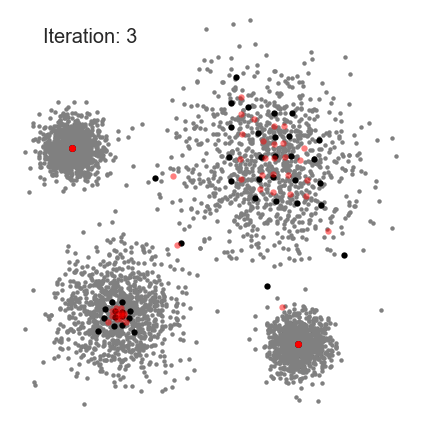
\includegraphics[scale=0.15]{meanshift/meanshift-10}\\
	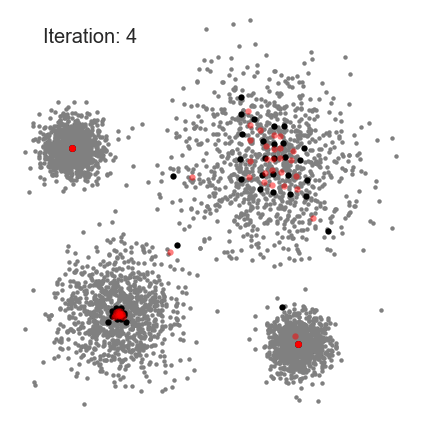
\includegraphics[scale=0.15]{meanshift/meanshift-12}&
	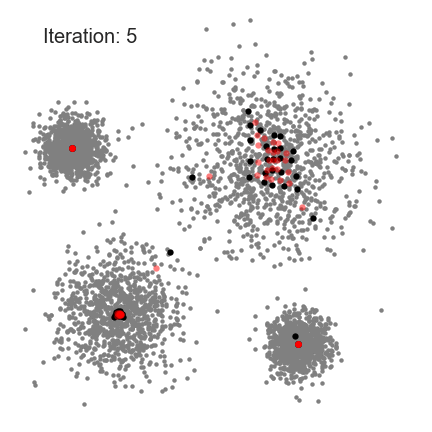
\includegraphics[scale=0.15]{meanshift/meanshift-14}&
	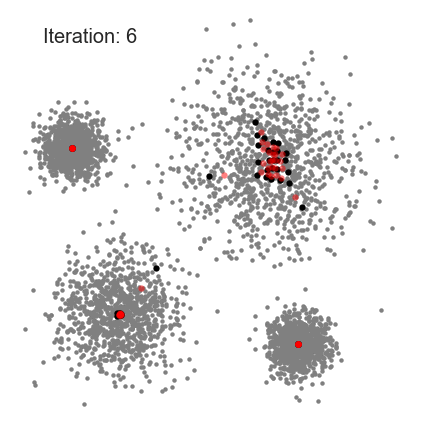
\includegraphics[scale=0.15]{meanshift/meanshift-16}&
	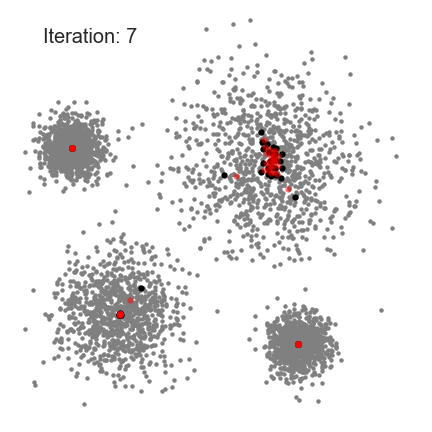
\includegraphics[scale=0.15]{meanshift/meanshift-18}&
	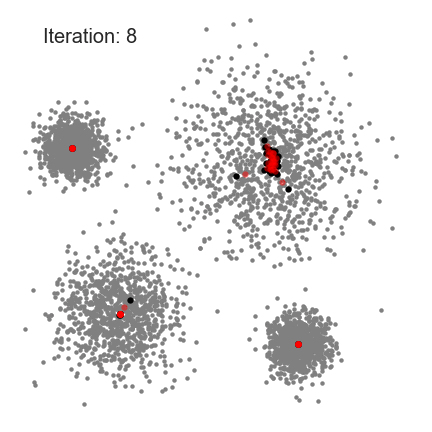
\includegraphics[scale=0.15]{meanshift/meanshift-20}\\
	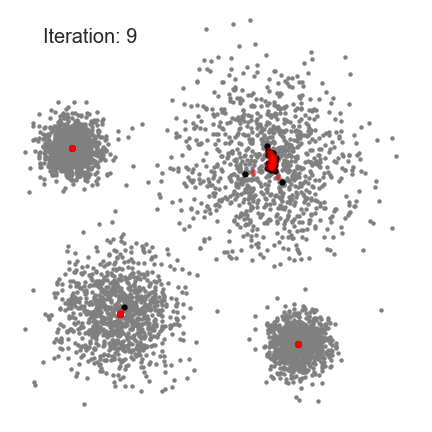
\includegraphics[scale=0.15]{meanshift/meanshift-22}&
	%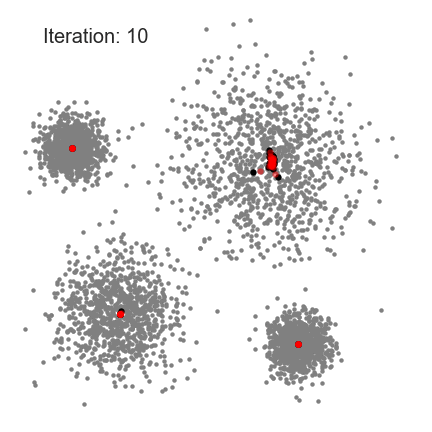
\includegraphics[scale=0.15]{meanshift/meanshift-24}&
	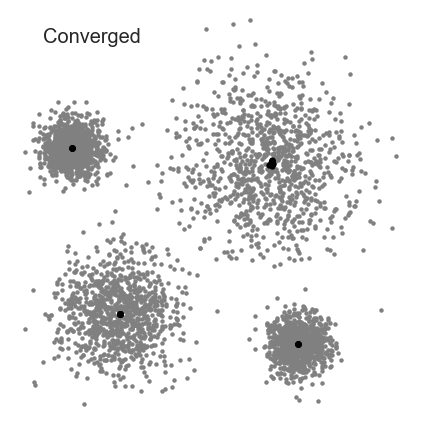
\includegraphics[scale=0.15]{meanshift/meanshift-36}&
	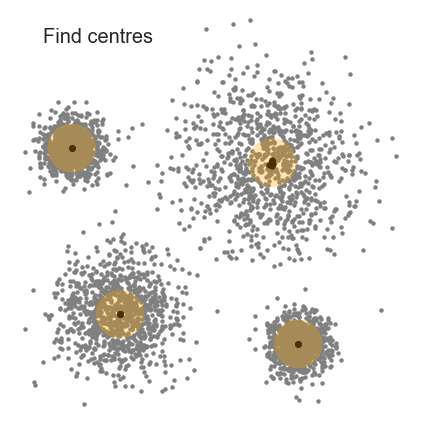
\includegraphics[scale=0.15]{meanshift/meanshift-38}&
	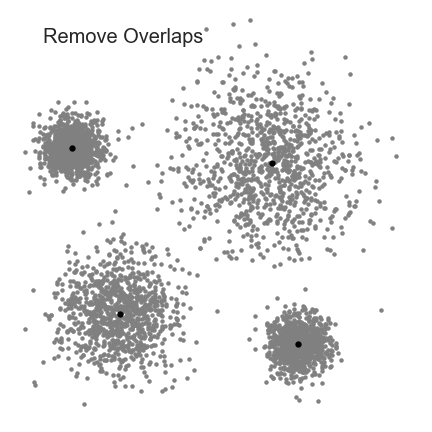
\includegraphics[scale=0.15]{meanshift/meanshift-40}&
	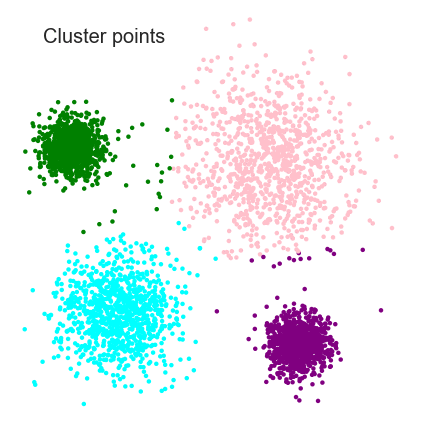
\includegraphics[scale=0.15]{meanshift/meanshift-43}\\
\end{tabular}
}
\end{frame}

\begin{frame}\frametitle{Density-Based Spatial Clustering of Applications with Noise-DBSCAN}
-label all data point to be unvisited. For all unvisited points:
	\begin{enumerate}
		\item All points which are within the $\epsilon$ distance are neighborhood points (part of the same cluster)
		\item If neighborhood points >= minPoints, then the clustering process starts and the current data point becomes the first point in the new cluster
		- Otherwise, mark the point as noise
		- In both cases that point is marked as “visited”
		\item repeated for all of the new points in the cluster group
		\item next an new unvisited point is retrieved and processed
	\end{enumerate}
Since at the end of this all points have been visited, each point will have been marked as either belonging to a cluster or being noise.

\end{frame}


\begin{frame}%\frametitle{dbscan}
\hspace*{-4pt}\makebox[\linewidth][c]{
	\begin{tabular}{cccc}
		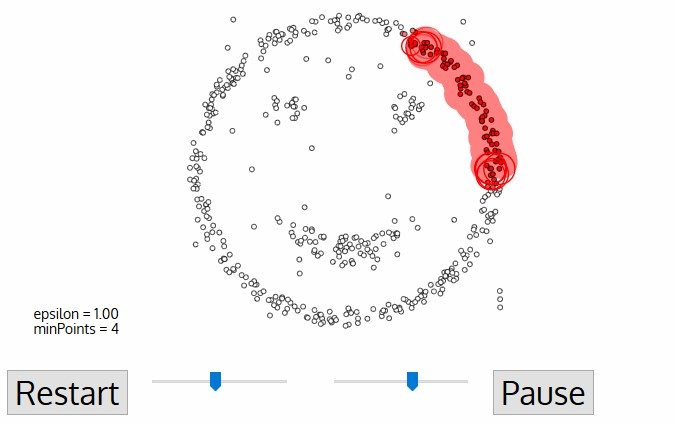
\includegraphics[scale=0.15]{dbscan/1}&
		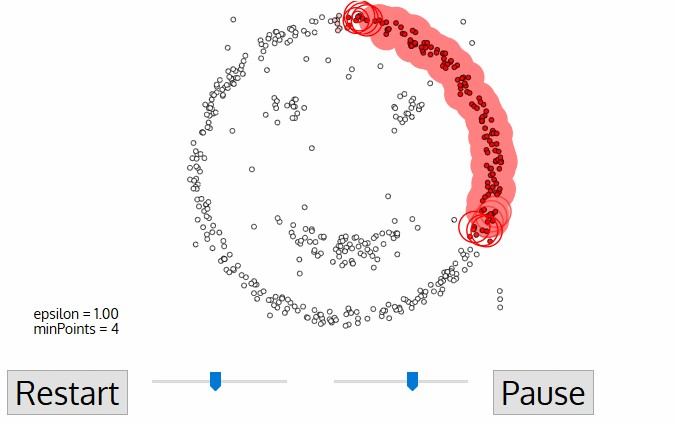
\includegraphics[scale=0.15]{dbscan/11}&
		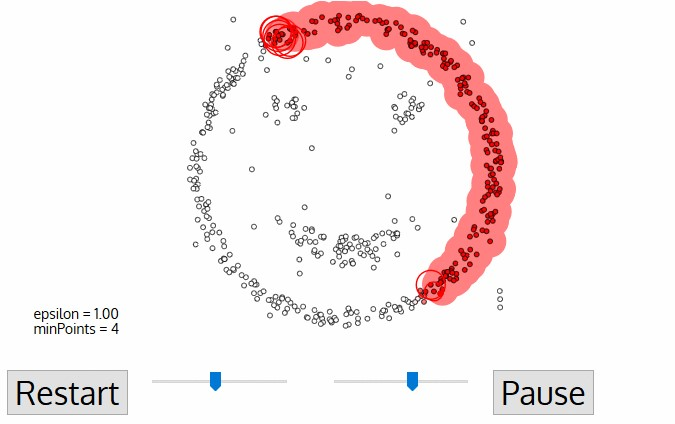
\includegraphics[scale=0.15]{dbscan/2}&
		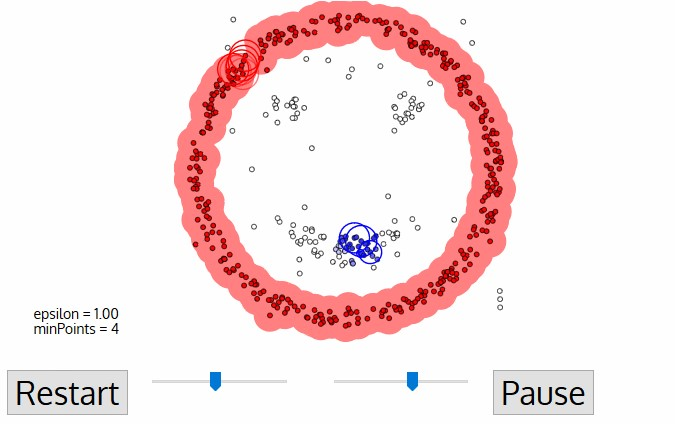
\includegraphics[scale=0.15]{dbscan/3}\\
		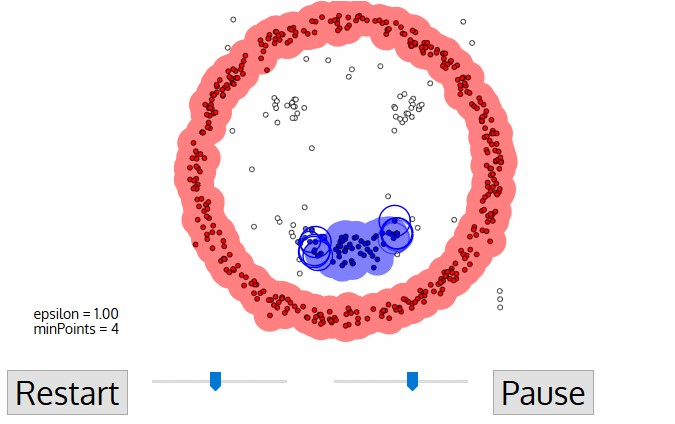
\includegraphics[scale=0.15]{dbscan/31}&
		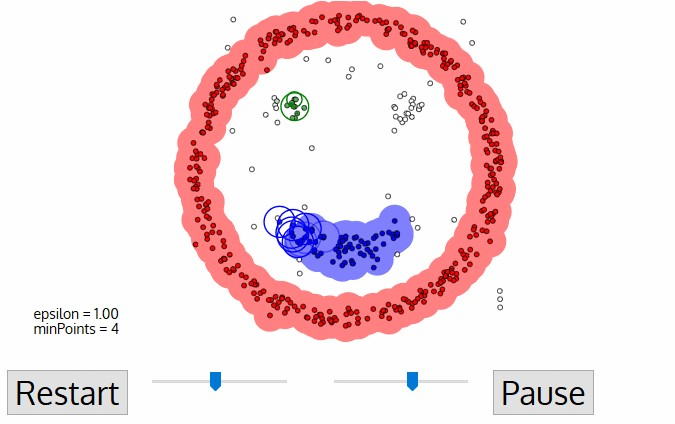
\includegraphics[scale=0.15]{dbscan/4}&
		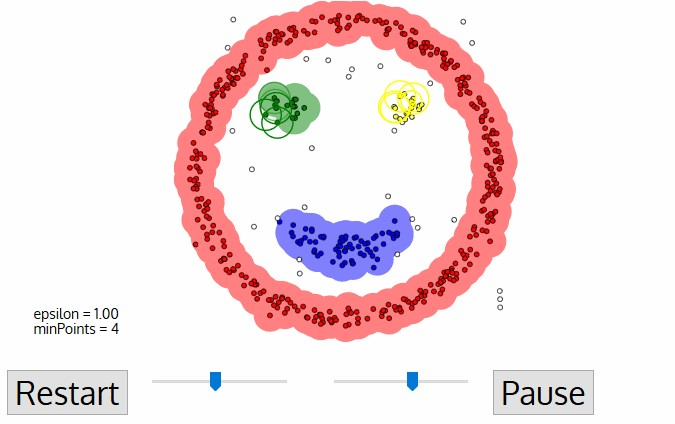
\includegraphics[scale=0.15]{dbscan/5}&
		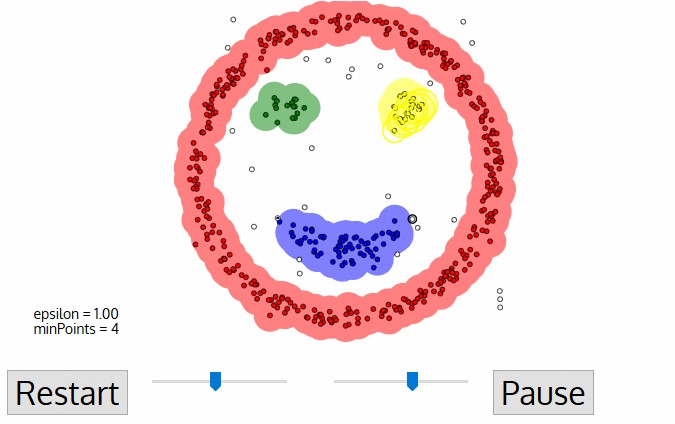
\includegraphics[scale=0.15]{dbscan/6}\\
		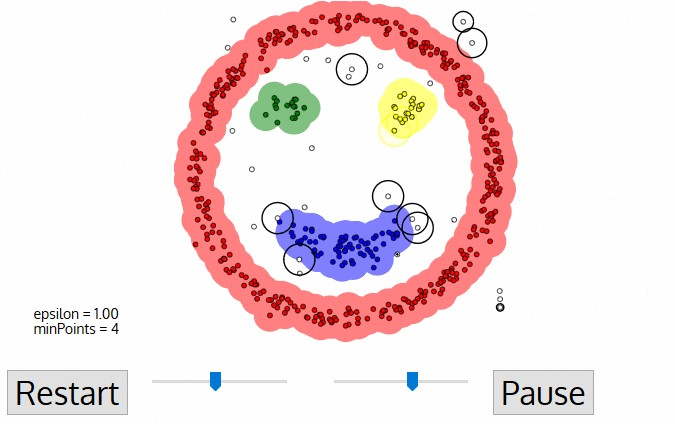
\includegraphics[scale=0.15]{dbscan/7}&
		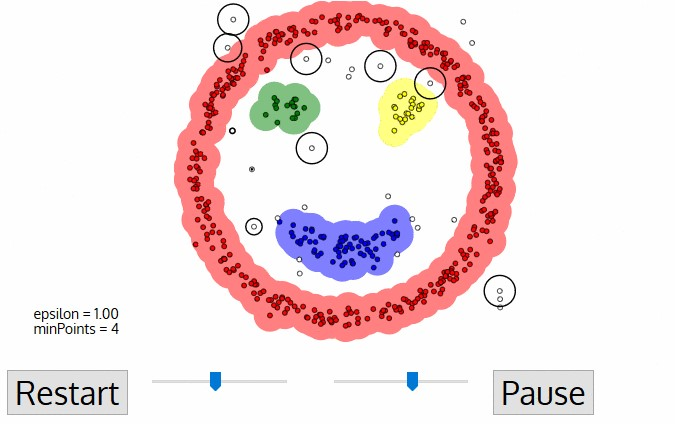
\includegraphics[scale=0.15]{dbscan/8}&
		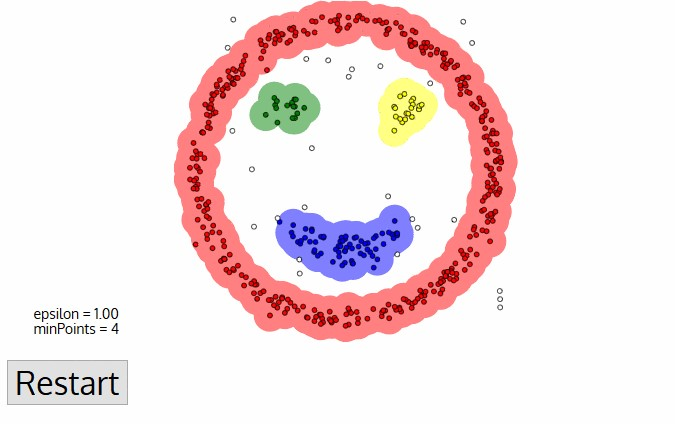
\includegraphics[scale=0.15]{dbscan/9}&
		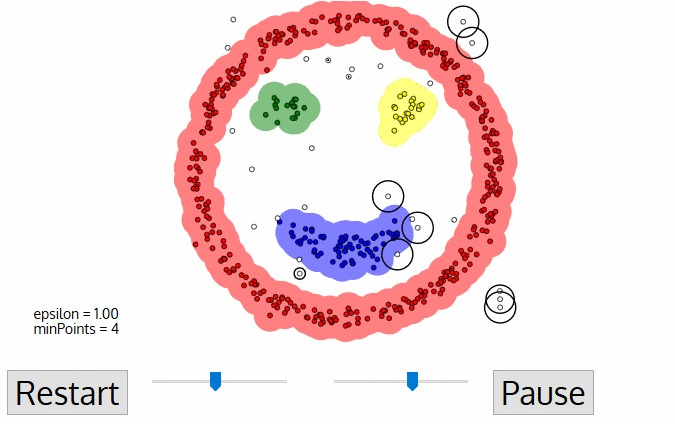
\includegraphics[scale=0.15]{dbscan/10}\\
	\end{tabular}
}
\end{frame}


\begin{frame}\frametitle{Hierarchical DBSCAN - HDBSCAN}
	content...
\end{frame}



\subsection{Distribution Models}
\begin{frame}\frametitle{Gaussian Mixture Models (GMMs)}
Assumption: the data points are Gaussian distributed (parameters: the mean and the standard deviation)! Each Gaussian distribution is assigned to a single cluster.
To find the parameters of the Gaussian for each cluster, use an optimization algorithm called Expectation–Maximization (EM). 

\end{frame}

\begin{frame}\frametitle{Expectation–Maximization (EM) using GMM}
choose num of clusters\\
compute the probability that each data point belongs to a particular cluster. With a Gaussian distribution we are assuming that most of the data lies closer to the center of the cluster.\\
From probabilities $\rightarrow$ recompute set of parameters such that we maximize the probabilities of data points within the clusters\\
We compute these new parameters using a weighted sum of the data point positions, where the weights are the probabilities of the data point belonging in that particular cluster.\\
Repeat till convergence\\

\end{frame}

\begin{frame}%\frametitle{EM}
\hspace*{-4pt}\makebox[\linewidth][c]{
\begin{tabular}{ccccc}
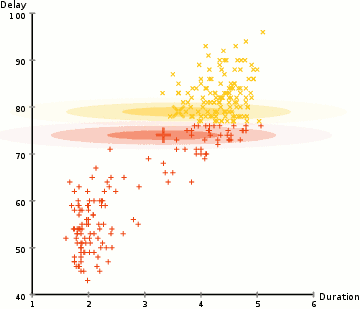
\includegraphics[scale=0.2]{em/frame_00_delay-0}&
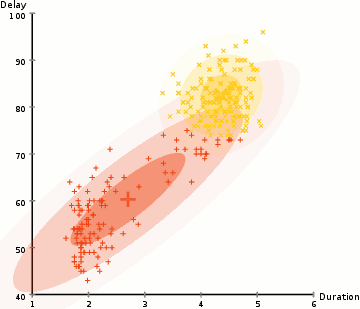
\includegraphics[scale=0.2]{em/frame_01_delay-0}&
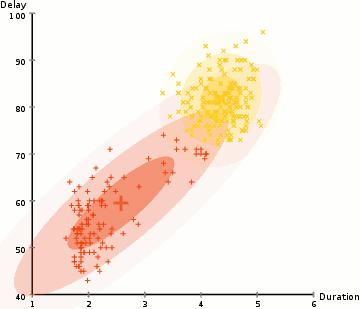
\includegraphics[scale=0.2]{em/frame_02_delay-0}&
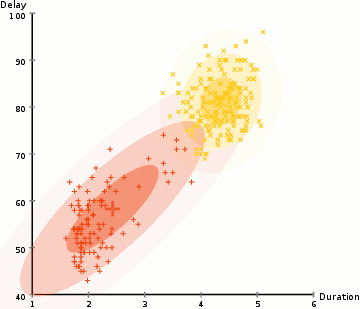
\includegraphics[scale=0.2]{em/frame_03_delay-0}&
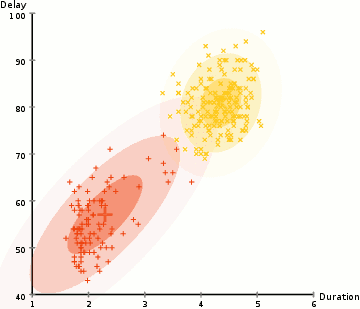
\includegraphics[scale=0.2]{em/frame_04_delay-0}\\
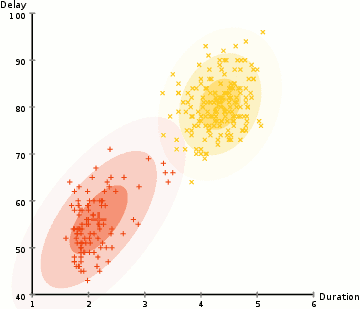
\includegraphics[scale=0.2]{em/frame_05_delay-0}&
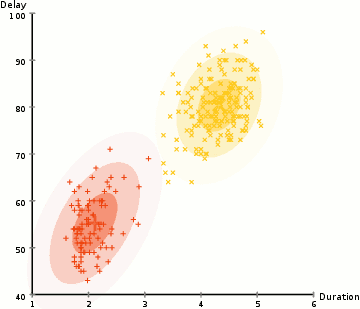
\includegraphics[scale=0.2]{em/frame_06_delay-0}&
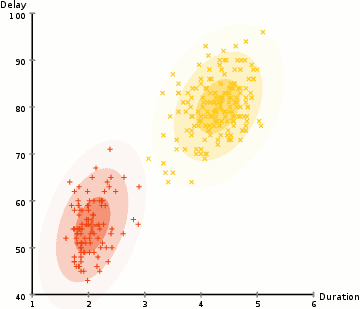
\includegraphics[scale=0.2]{em/frame_07_delay-0}&
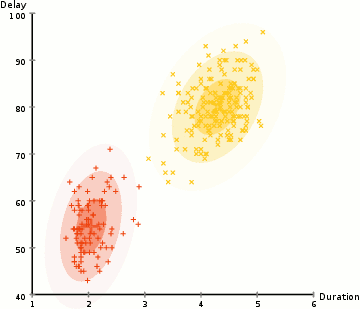
\includegraphics[scale=0.2]{em/frame_08_delay-0}&
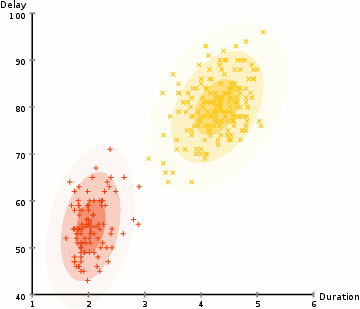
\includegraphics[scale=0.2]{em/frame_09_delay-0}\\
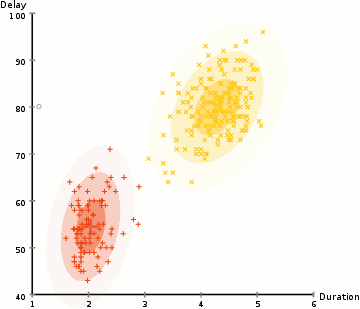
\includegraphics[scale=0.2]{em/frame_10_delay-0}&
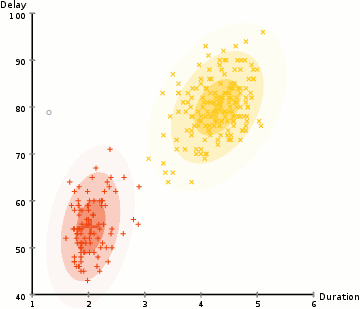
\includegraphics[scale=0.2]{em/frame_11_delay-0}&
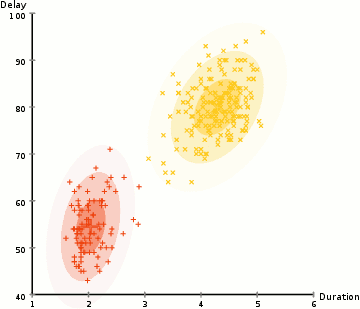
\includegraphics[scale=0.2]{em/frame_12_delay-0}&
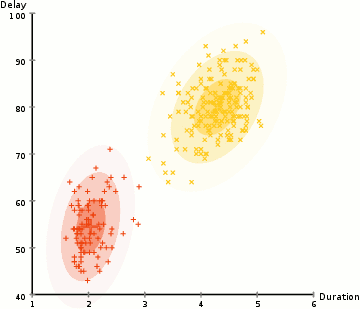
\includegraphics[scale=0.2]{em/frame_13_delay-0}&
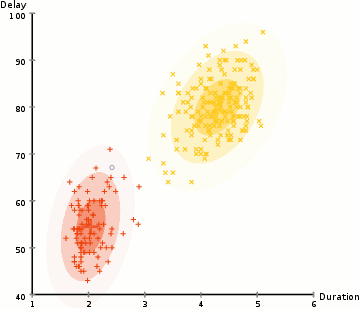
\includegraphics[scale=0.2]{em/frame_14_delay-0}\\
\end{tabular}
}
\end{frame}


\subsection{Centroidal models}
\begin{frame}\frametitle{K means}
iterative clustering algorithm that aims to find local maxima in each iteration\\
take a quick look at the data and choose k (num clusters)\\
assign data points to the cluster $\leftrightarrow$
compute cluster centroid\\
repeat to reduce variation error\\
elbow method
\begin{columns}
	\begin{column}{.5\textwidth}
		\includegraphics[scale=0.5]{kmeans_1}
	\end{column}
	\begin{column}{.5\textwidth}
		\includegraphics[scale=0.2]{kmeans_2}
	\end{column}
\end{columns}
\end{frame}



\begin{frame}\frametitle{k-median}
\textbf{K median vs kmeans}: instead of recomputing the group center points using the mean (like in K-Means) we use the median vector of the group. This method is \textbf{less sensitive to outliers} (because of using the Median) but is \textbf{much slower for larger datasets as sorting is required} on each iteration when computing the Median vector\\
\textbf{mean-shift vs kmeans}: Instead of selecting the number of clusters as mean-shift automatically discovers this (advantage), the selection of the window size/radius “r” can be non-trivial.

\end{frame}


\begin{frame}\frametitle{kmeans fail}
	\includegraphics[scale=0.5]{kmeans_fail}\\
	K-Means is actually a special case of GMM in which each cluster’s covariance along all dimensions approaches 0
\end{frame}



\subsection{Connectivity Models}
\begin{frame}\frametitle{Agglomerative Hierarchical Clustering}
The decision of dividing into or merging \textbf{two} clusters is taken on the basis of closeness of these clusters. Metrics for deciding the closeness of two clusters:\\
Euclidean distance: $||a-b||_2=\sqrt{\sum(a_i-b_i)}$\\
Squared Euclidean distance: $||a-b||_2^2=\sum(a_i-b_i)^2$\\
Manhattan distance: $||a-b||_1=\sum|a_i-b_i|$\\
Maximum distance: $||a-b||_{INFINITY} =\max_i|a_i-b_i|$\\
Mahalanobis distance: $\sqrt(a-b)^T S^{-1} (-b)$\\
Maybe, use \textbf{average linkage} which defines the distance between two clusters to be the average distance between data points in the first cluster and data points in the second cluster.

\end{frame}


\begin{frame}\frametitle{hierarchical agglomerative clustering (HAC) or bottom-up}

\begin{enumerate}
	\item Each data point as a single cluster
	\item select a distance metric 
	\item Iterate till convergence\\
	 - combine two clusters with the smallest average linkage
\end{enumerate}



\begin{columns}
	\begin{column}{0.3\textwidth}
		\includegraphics[scale=0.25]{hierarchical}
	\end{column}
	\begin{column}{0.65\textwidth}
		
		The height in the dendrogram at which two clusters are merged represents the distance between two clusters in the data space.\\
		take 4 clusters as the red horizontal line in the dendrogram covers maximum vertical distance AB.\\
		
		
	\end{column}
\end{columns}

\end{frame}













%%%%%%%%%%%%%%%%%%%%%%%%%%%%%%%%%%%%%%%%%%%%%%%%%%%%%%%%%%%%%%%%%%%%%%%%%%%%%%%%%%%%%%%%%%%%%%%%%%%%%%%%%%%%%%%%%%%%%%%%%%%%%%%%%%%%%%%%%%




\section{ML Techniques}


\subsection{SVM}

\begin{frame}\frametitle{Support Vector Machines}
	what are support vectors?\\
	which kernel (linear, radial, polynomial,sigmoid/logistic, gaussian/RBF - radial basis func)\\
	can handle categorical/numerical data?\\
	In a N-dimensional Euclidean space, plot a hyper-plane $\Rightarrow$ (n-1) dim subset of n-dimensional Euclidean space dividing it into 2\\
	\begin{alertblock}{sklearn code}
		clf = sklearn.svm.SVC(kernel='linear')\\
		clf.fit(X,y)\\
		clf.predict([])
	\end{alertblock}
	C: smooth decision boundary (C$\downarrow$) \& classified training points (C$\uparrow$)\\
	Gamma: $\uparrow \gamma \Rightarrow$ points closer to hyperplance will have more wt
\end{frame}


\subsection{Ensemble}

\begin{frame}[allowframebreaks]%[plain]
	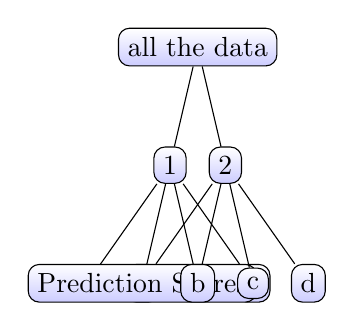
\begin{tikzpicture}[
		sibling distance=2em,
		every node/.style = {
			shape=rectangle, rounded corners,
			draw, align=center,
			top color=white, bottom color=blue!20}]]
		\node {all the data}
			child { node {1}
					child { node {a} }
					child { node {b} }
					child { node {c} }
					child { node {d} }
			}
			child { node {2}
				child { node {Prediction Scores} }
				child { node {b} }
				child { node {c} }
				child { node {d} }
			}
			;
	\end{tikzpicture}\\
	DT = Low bias high variance\\
	Uses:\\
	\begin{itemize}
		\item D$^3$ algo
		\item Entropy ($-p \log_2 p - q \log_2 q$)
		\item Information Gain
	\end{itemize}
Gini impurity or entropy? The truth is, most of the time it does not make a big difference: they lead to similar trees. Gini impurity is slightly faster to compute, so it is a good default. However, when they differ, Gini impurity tends to isolate the most frequent class in its own branch of the tree, while entropy tends to produce slightly more balanced trees.\\
\textbf{Linear Model vs decision trees}:\\
linear models make assumptions... dec trees may over-fit
LM $\Rightarrow$ parametric (predetermined number of parameters $\Rightarrow$ limited degree of freedom $\Rightarrow$ reducing the risk of overfitting (but increasing the risk of underfitting)
DT $\Rightarrow$ non-parametric (number of parameters is not determined prior to training) $\Rightarrow$ over-fitting\\
Standard statistical tests, such as the $\chi^2$ test, are used to estimate the probability that the improvement is purely the result of chance (H$_0$). If this probability, called the pvalue, is higher than a given threshold (typically 5\%, controlled by a hyperparameter), then the node is considered unnecessary and its children are deleted. The \textbf{pruning} continues until all unnecessary nodes have been pruned\\
cons of decision tree: orthogonal boundaries, not a good model; sensitive to small variations;\\
Voting classifiers: hard voting (majority-vote classifier) \& soft voting\\
even if each classifier is a weak learner (meaning it does only slightly better than random guessing), the ensemble can still be a strong learner (achieving high accuracy), provided there are a sufficient number of weak learners and they are sufficiently diverse.\\
this is only true if all classifiers are perfectly independent, making uncorrelated errors, which is clearly not the case since they are trained on the same data. They are likely to make the same types of errors, so there will be many majority votes for the wrong class, reducing the ensemble’s accuracy.\\
Ensemble methods work best when the predictors are as independent from one another as possible. One way to get diverse classifiers is to train them using very different algorithms. This increases the chance that they will make very different types of errors, improving the ensemble’s accuracy.
\end{frame}


\begin{frame}\frametitle{Sequential - Boosting}
	\begin{itemize}
		\item adaptive Boosting:\\
		start with equal wt to decision stump, then misclassified gets higher weights for the next decision stump
		\item Gradient Boosting:\\
		optimize loss funct of prev learner\\
		additive model regularize the loss function
		\item XG Boosting: extreme gradient\\
		computational speed and model efficiency\\
		distributed ML: create decision tree $\parallel$-ly\\
		out of core computing\\
		cache optimization\\
		$\uparrow$ bias, $\downarrow$ variance\\
		uses DT upto some depth
	\end{itemize}
\end{frame}

\begin{frame}\frametitle{\hypertarget{rf}{Parallel - Bagging - Random Forest}}
	DT = $\downarrow$ bias, $\uparrow$ variance\\
	RF = DT1 + DT2 + ...\\
	   = $\downarrow$ bias, $\downarrow$ variance\\
	classification = votes\\
	regression = average
\end{frame}

\begin{frame}\frametitle{Stacking}
	content...
\end{frame}

%%%%%%%%%%%%%%%%%%%%%%%%%%%%%%%%%%%%%%%%%%%%%%%%%%%%%

\section{Python Libraries}
\subsection{scikit-learn}

\begin{frame}\frametitle{Training-stochastic}
training algorithm used by Scikit-Learn : stochastic; may
get very different models even on the same training data (unless you set the random\_state hyperparameter).
\end{frame}

%%%%%%%%%%%%%%%%%%%%%%%%%%%%%%%%%%%%%%%%%%%%%%%%%%%%%



\section{Time Series}
\begin{frame}\frametitle{Trend Analysis}
	content...
\end{frame}	

\begin{frame}[allowframebreaks]\frametitle{ARIMA Modeling}
	Auto-regressive Integrated Moving Average\\
	\begin{enumerate}
		\item AR Model (p)\\
		\item MA Model (q)\\
		\item ARMA Model (p,q)\\
		\item \textbf{ARIMA(p,d,q)}\\	
		\item \textbf{SARIMA(p,d,q)(P,D,Q)$_m$}
		\begin{enumerate}
			\item S [(P,D,Q)$_m$]: Seasonality; m = Seasonality; (P,D,Q) are analogous of (p,d,q) except for seasonal components\\
			\textbf{what is Seasonality?} Repeating patterns within a year (/weekly/monthly). Remove Seasonality:\\
			\begin{alertblock}{Math alert}
				$Z_t = S_{t-365}-S_t$ \\
			\end{alertblock}
	
			\textbf{What is Cycle?}: 
			\begin{itemize}
				\item repeating patterns over years
				\item not as predictable, I cycle might take 2 years, II might take 3 years, III might take 2.5 years
			\end{itemize}
			\item AR [p]: predict for today based on previous value
			\item I [d]: TS has forwards or backwards trends, so use differencing to make it stationary\\
			\begin{alertblock}{Math alert}
				$Z_t = S_{t-1}-S_t = \phi Z_{t-1} + \theta \epsilon_{t-1} + \epsilon_t $\\
				To Recover, $S_k = Z_{k-1}+S_{k-1} = \sum_{i=1}^{l}Z_{k-i} + S_l$\\				
			\end{alertblock}
			\item MA [q]: error from prev period t make prediction about today
			\begin{alertblock}{Math alert}
				Actual, $X_t = \mu + \phi_1\epsilon_{t-1} + \phi_2\epsilon_{t-2} + ... + \phi_q\epsilon_{t-q} + \epsilon_t $\\
				Pred, $\hat{X}_t = \mu + \phi_1\epsilon_{t-1} + \phi_2\epsilon_{t-2} + ... + \phi_q\epsilon_{t-q} $ (won't account for error)\\
				where,\\
				$\epsilon_{t-q}$ and $\epsilon_t$ : error from q time periods ago and current time period\\
				$S_t, S_{t-1}, S_{t-2}$: avg value @t, t-1, t-2\\
				\textbf{ACF}: Auto-correlation factor = Corr($S_{t-2}, S_t$)\\
			\end{alertblock}
			Pearson's r correlation: measures the strength relation btw	2 variables\\
		\end{enumerate}
		AR $\Rightarrow$ regression $\Rightarrow$ auto regression (predict something based on past values of same "something") (PACF)\\
		MA $\Rightarrow$ (ACF)\\
	\end{enumerate}	
\end{frame}	

\begin{frame}\frametitle{Trend Analysis}
content...
\end{frame}	

\begin{frame}\frametitle{Trend Analysis}
content...
\end{frame}	

\begin{frame}\frametitle{Trend Analysis}
content...
\end{frame}	

\begin{frame}
Thank You!
\end{frame}


\end{document}